\chapter{Introdução}

\subsection*{\textbf{Por que cidades existem?}}

Para Bauman, cidades são lugares de oportunidades e são movidas por ``newcomers'', pessoas que não são originalmente do lugar e são estranhos à sua realidade. Quando essas pessoas chegam nas cidades, elas apresentam novas perspectivas sobre problemas antigos e suas formas de pensar geralmente conflitam com tranquilidade consequente da familiaridade e convivência dos residentes bem estabelecidos. Apesar disso poder gerar incômodo aos nativos, é para o bem deles e da cidade que suas formas de ser sejam questionadas e desafiadas pelos estranhos. Para o autor, esse estado de inquietude e permanente sentimento de ``ser estrangeiro'' é o que leva as pessoas e a cidade a buscar reflexão, debate e inovação \cite{bauman2003city}.

Para Jane Jacobs, uma característica que determina o sucesso de uma cidade é sua vitalidade. A autora defendia que a vida na cidade depende fortemente das dinâmicas sociais, das interações cotidianas de seus residentes. Para Jacobs, a cidade proporciona interações nos espaços públicos -- onde a vida urbana efetivamente acontece -- e possibilita que as pessoas se conectem, encontrem, colaborem e prosperem juntas. Ela valorizava a diversidade, densidade e a mistura de usos do solo urbano, argumentando que a presença de uma variedade de estabelecimentos comerciais, residenciais e culturais em uma mesma área promove a interação entre diferentes grupos sociais e estimulava a criatividade e a inovação \cite{jacobs1961death}.

Do ponto de vista econômico, o triunfo da cidade se encontra nos benefícios de aglomeração e adensamento. Economias de aglomeração permitem que firmas diferentes escolham ficar geograficamente próximas umas das outras e encontrem benefício econômico ao reduzirem seus custos e aumentarem a produtividade. Jan Brueckner, em \textit{Lectures on Urban Economics}, delimita no capítulo 1 o racional econômico da existência de cidades, que se divide em quatro principais componentes.

A aglomeração tecnológica $(i)$ aumenta a produtividade dos trabalhadores, na medida em que os empregos são mais concentrados e há ``transbordamento'' de conhecimento entre as firmas da região. Além disso, uma oferta maior e mais diversa de trabalho, causa maior competitividade e eficiência na escolha da pessoa certa para cada cargo. Aglomerações pecuniárias $(ii)$ reduzem os custos das firmas, sem alterar sua produtividade. Com maior demanda por serviços como segurança, limpeza, contratação e advocacia, estes mercados se desenvolvem, tornam-se mais competitivos, eficientes e baratos. Inclusive, há serviços especializados de nicho, que podem estar disponíveis e acessíveis apenas em grandes centros urbanos. Aglomeração de varejo $(iii)$ traz ganhos para os consumidores e comerciantes. Quando o comércio está aglomerado, o consumidor pode escolher entre mais opções e se desloca menos entre seus destinos caso queria comprar mais de um item. Dessa forma, os consumidores ganham e os comerciantes também, visto que com mais consumidores e maior fluxo, maiores as vendas. Por fim, o custo de transporte $(iv)$ é um dos fatores que mais mudam quando há densidade. A redução do custo de transporte, que pode ser considerada uma economia de aglomeração pecuniária, acontece não apenas para os trabalhadores, que se deslocam menos às oportunidades de emprego, mas também às firmas que gastam menos transportando seus bens e serviços \cite{brueckner2011lectures}.

Nesse sentido, se aglomeração e densidade trazem benefícios, uma cidade bem sucedida é uma cidade que ao longo do tempo tende a se adensar cada vez mais. Entretanto, uma pergunta relevante é se as forças de aglomeração atuam sozinhas ou se precisam de incentivos e regulação. Os modelos de economia urbana demonstram que as próprias forças de mercado agem de forma a incentivar o adensamento, mas há fatores que podem atuar na direção contrária também \cite{brueckner2011lectures} -- mais detalhes serão discutidos na Seção \ref{sec:micro}. Nessa perspectiva, a função das instituições seria de intervir de forma a combater essas forças, apoiando o adensamento. 

Por outro lado, Edward Glaeser em \textit{Triumph of the City} discute alguns desafios encontrados pela regulamentação e incentivos criados pelas insituições. Segundo o autor, muitas vezes a regulamentação apresenta procedimentos lentos e burocráticos, e acaba gerando decisões focadas em fatores que se sobrepõem o adensamento na escala de prioridades. Inclusive, o que Glaeser propõe é criar impostos \textit{à la} Coase, de forma que os incentivos se alinhem para uma cidade mais densa, ainda compensando pelos seus possíveis malefícios. 

Ronald Coase reconhece natureza recíproca do problema do custo social, no caso em que A causa malefícios a B, mas B também causa malefícios a A. Isso se aplica a um exemplo em que uma empresa (A) quer construir um prédio, mas a comunidade local não quer ser perturbada mudanças na região. Caso a empresa (A) siga com a construção, a comunidade local (B) será prejudicada, mas se a construção for barrada, a empresa (A) também sofrerá e menos oferta habitacional e empregos serão gerados. Coase propõe uma forma de pensar que leva em conta não apenas a ponderação de qual malefício é maior, mas também a compensação da parte que sai prejudicada de um eventual acordo. Dessa forma, é sempre feita a escolha que maximize o bem-estar social, sem causar distorções nas escolhas, ainda compensando a parte prejudicada \cite{coase2013problem}.

\begin{quotation}
   ``Primeiro, as cidades devem substituir seus longos e incertos procedimentos de licenciamento com um simples sistema de taxação. Se prédios altos criam custos ao bloquear vistas ou luz, então faça uma estimativa razoável desses custos e cobre o construtor de acordo. Se certas atividades são nocivas aos vizinhos, então devemos estimar o custo social e cobrar os construtores por eles, assim como devemos cobrar motoristas pelos custos de gerar engarrafamentos. Esses impostos podem então ser dados às pessoas que estão sendo impactadas, como os vizinhos que perderam a iluminação por um novo prédio que obstrui sua vista.'' \cite{glaeser2011triumph}

\end{quotation}

\subsection*{\textbf{Regulamentação em São Paulo}}

Atualmente em São Paulo, os mecanismos de regulação são principalmente definidos pelo atual Plano Diretor Estratégico de SP \cite[PDE]{PDE}. No código da lei do PDE, entre os 17 objetivos estabelecidos, ao menos nove estão relacionados a estratégias de adensamento urbano \cite{lima2021alem}. A ideia principal do plano é direcionar o adensamento para áreas capazes de admitir um grande volume de habitantes, principalmente no entorno de infraestruturas de transporte de alta capacidade.

O PDE institui uma variedade de instrumentos para gerar esse adensamento, alguns atuando sobre empreendimentos já existentes, e outros para os novos também. O artigo 96 do PDE estabelece que ``os imóveis não edificados, subutilizados e não utilizados são sujeitos ao parcelamento, edificação e utilização compulsórios'', de forma a passar a exercer sua função social dentro de um prazo estabelecido. Existem, inclusive, dispositivos para lidar especificamente com imóveis com este perfil em áreas que dispõem das características apropriadas para um maior adensamento, como é o caso das ZEIS 3:

\begin{quotation}
    ``ZEIS 3 são áreas com ocorrência de imóveis ociosos, subutilizados, não utilizados, encortiçados ou deteriorados localizados em regiões dotadas de serviços, equipamentos e infraestruturas urbanas, boa oferta de empregos, onde haja interesse público ou privado em promover Empreendimentos de Habitação de Interesse Social''

    \raggedleft Art. 45 do PDE \cite{PDE}
\end{quotation}

Para a regulação dos novos empreendimentos, há três principais dispositivos. O primeiro deles é o gabarito, que determina a altura máxima, em metros, dos imóveis. Outro instrumento é o coeficiente de aproveitamento (CA), que determina quantas vezes a área do lote pode ser construída. Se o CA é básico (CA = 1), e o lote possui 1.000m$^2$, então pode ser construído um empreendimento que distribui estes 1.000m$^2$ em uma quantidade qualquer de andares que respeite o gabarito. Se o CA for 2, significa que para o mesmo lote, podem ser distribuídos 2.000m$^2$ em \textit{n} andares. Por fim, a cota parte é a cota máxima de terreno por unidade habitacional e determina o número mínimo de unidades habitacionais do terreno. Para calcular a cota parte, basta dividir o lote pelo número de unidades, resultando na cota do terreno ocupada por cada unidade habitacional. Dessa forma, o número mínimo de unidades habitacionais é dado pela Equação \ref{eq:cotaparte}, na qual $A_t$ representa a área do lote e $Q$ a cota parte.

\begin{equation}
    N_{min} = \frac{\text{CA}_{\text{utilizado}}}{\text{CA}_{max}}\cdot \frac{A_t}{Q}
    \label{eq:cotaparte}
\end{equation}

No PDE, foram estabelecidos diferentes níveis de CA na cidade, a depender dos objetivos que se tem em relação à região, como é possível observar na Figura \ref{fig:CA}. Nas regiões de preservação ambiental, por exemplo, o CA é de 0.1, o menor da cidade, enquanto nas áreas do entorno de equipamentos de transporte pública de alta capacidade, (EETUs), o CA chega a 4. Com isso, o adensamento é direcinado às áreas que são aptas a receber mais habitantes.

\begin{figure}[h]
    \caption{Coeficientes de aproveitamento (CA) na cidade}
    \label{fig:CA}
    

    \caption*{\raggedright \textbf{Macroáreas}}
    \begin{subfigure}{.9\textwidth}
        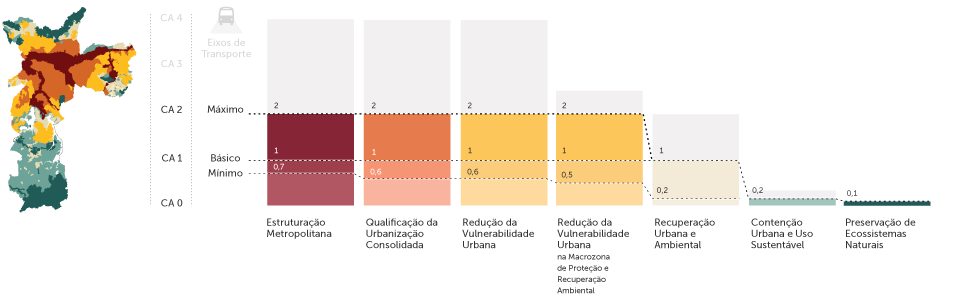
\includegraphics[width = \textwidth]{imagens/CA_macroareas.png}
    \end{subfigure}

    \caption*{\raggedright \textbf{Eixos de Estruturação da Transformação Urbana (EETU)}}
    \begin{subfigure}{.9\textwidth}
        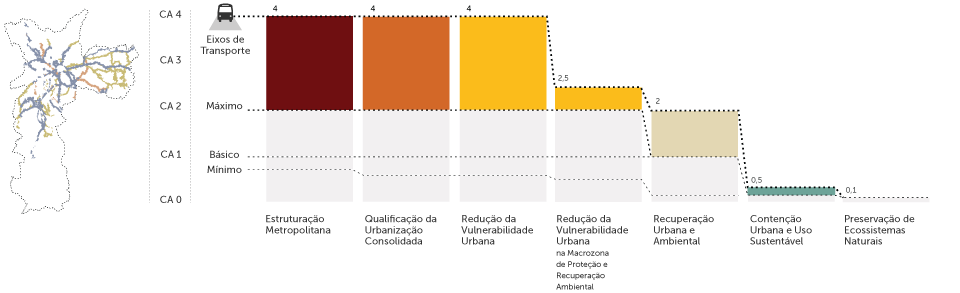
\includegraphics[width = \textwidth]{imagens/CA_eixos.png}
    \end{subfigure}
    \caption*{Fonte: \url{https://gestaourbana.prefeitura.sp.gov.br/marco-regulatorio/plano-diretor/entenda-o-projeto-de-lei-68813/}}
\end{figure}

Da mesma forma, existem parâmetros para a cota parte na cidade, a depender da localização. Nas Macrozonas de Estruturação e Qualificação Urbana, por exemplo, a cota parte apontada na Equação \ref{eq:cotaparte} como $Q$ equivale a 20. Em termos práticos, isso significa que um lote de 1.000m$^2$ hipotético deve apresentar no mínimo 50 unidades habitacionais. Este valor não é incrementado por um aumento do CA, mas pode decrescer se o CA escolhido pelo projeto seja menor do que o CA máximo da região.

Nesse sentido, não existe exatamente um dispositivo que determine a densidade populacional em si. Isso pode levar a um cenário em que o mercado está fracamente regulado, implicando que a densidade não está sendo efetivamente decidia pelo PDE. Apesar de haver um número mínimo de unidades habitacionais, estas não necessariamente se traduzem em população, dado que ao mesmo tempo que pode abrigar uma única pessoa, também pode abrigar uma família com diversos membros. Além disso, este valor mínimo não é afetado pela verticalização do imóvel, então imóveis com um CA maior não são obrigados a terem mais unidades habitacionais.

\subsection*{\textbf{O problema}}

Levando em consideração que um dos principais objetivos do PDE é estimular o adensamento de determinadas áreas, é importante avaliar se os instrumentos de regulação que estão disponíveis para alcançar este objetivo são eficientes. Em outras palavras, é crucial entender se os 3 components expostos (CA, cota parte e gabarito) são suficientes para determinar a densidade populacional que um novo empreendimento vai gerar. 

Caso estes instrumentos apontados não sejam eficientes em determinar a densidade, o nível de adensamento estaria sendo decidido pelo mercado. Entretanto, o que é importante notar é que o mercado sempre busca maximizar seus lucros, o que não necessariamente reflete em maior densidade populacional. Do ponto de vista teórico, é importante compreender quais elementos estão envolvidos nas escolhas das firmas na oferta de unidades de habitação, que será uma discussão da Seção \ref{sec:micro}.

Na Seção \ref{sec:emp}, será avaliado se estes instrumentos determinam a densidade demográfica. Para tanto, serão usados os dados do IPTU para calcular os indicadores utilizados na regulação e os dados do Censo de 2022, para identificar a densidade demográfica da região. Caso os indicadores sejam suficientes para explicar a densidade, significa que o PDE consegue definir a densidade usando os instrumentos previstos na lei. Caso contrário, a densidade populacional está sendo efetivamente decidida via mercado, não estando necessariamente alinhada com os objetivos do Plano para a cidade.

\chapter{Teórico}
\label{sec:micro}


\chapter{Empírico}
\label{sec:emp}